%-------------------------------------------------------------------------
%\documentclass[11pt,authoryear]{elsarticle}
\documentclass[authoryear,11pt]{elsarticle}


\setlength{\parskip}{1em}			% espaciar parrafos
\newtheorem{proposition}{Proposition}
\newtheorem{definition}{Definition}
\newtheorem{proof}{Proof}
\newtheorem{corollary}{Corollary}

\usepackage{hyperref}				% enlaces en el pdf
\hypersetup{backref,colorlinks=true}	% colores en vez de cajas en los enlaces
\usepackage{times}              		% la letra
\usepackage{graphicx}           		% para manejar imagenes
\usepackage{subfigure}          		% para manejar subfiguras
\usepackage{tabularx}		   		% para ajustar el ancho de las columnas
\usepackage[margin=2.5cm]{geometry}	% Change margins
\usepackage[table]{xcolor}			% Colores en el cronograma
\usepackage{multirow}				% Cabecera del cronograma
\usepackage{watermark}				% Para la portada
\usepackage{datetime}				% Fecha de creado
\usepackage{pst-tree}				% Para la taxonomía
\usepackage{stackengine}				% Para listar los articulos en el nodo de la taxonomía
\usepackage{algorithm}				% Para el seudocódigo
\usepackage{setspace}				% Para el seudocódigo
\usepackage{amsmath}					% Para el seudocódigo
\usepackage[noend]{algpseudocode}	% Para el seudocódigo
\usepackage{multicol}				% Para el seudocódigo


\newcolumntype{L}[1]{>{\raggedright\let\newline\\\arraybackslash\hspace{0pt}}m{#1}}
\newcolumntype{C}[1]{>{\centering\let\newline\\\arraybackslash\hspace{0pt}}m{#1}}
\newcolumntype{R}[1]{>{\raggedleft\let\newline\\\arraybackslash\hspace{0pt}}m{#1}}

%-------------------------------------------------------------------------
% Configuring Taxonomy
%-------------------------------------------------------------------------
\setstackEOL{\\}
\def\psedge{\ncangles[angleA=-90,angleB=90]}
\psset{levelsep=20mm,treesep=1cm,nodesep=3pt, arrows=->}
\def\PSBL#1{\small\pspicture(7,0.8)\psTextFrame[shadow,
  fillstyle=solid,linecolor=blue,framearc=0.3](0,0)(7,0.8){%
    \shortstack{#1}}\endpspicture}
\def\PSBS#1{\pspicture(3,.7)\psTextFrame[shadow,
  fillstyle=solid,linecolor=blue,framearc=0.3](0,0)(3,0.8){%
    \shortstack{#1}}\endpspicture}

%-------------------------------------------------------------------------
% Referencias a una palabra
%-------------------------------------------------------------------------
\newcommand{\setword}[2]{%
  \phantomsection
  #1\def\@currentlabel{\unexpanded{#1}}\label{#2}%
}


\begin{document}
	
	\title{Development of fast algorithms for reduct computation}
	
	\author{Vlad\'imir Rodr\'iguez Diez}
	\author{Jos\'e Francisco Mart\'inez Trinidad}
	
	\address{Computer Science Department\\National Institute of
	Astrophysics, Optics and Electronics\\
	Luis Enrique Erro \# 1, Santa Mar\'{\i}a Tonantzintla, Puebla,
	72840, M\'{e}xico} 
%	\email{\{vladimir.rodriguez,fmartine\}@inaoep.mx}
	
	
%	\thispagestyle{empty}
	
%	\begin{abstract}
%		Information systems in Rough Set Theory (RST) are tables of objects described by a set of attributes. 
%		This type of tables are widely used in different pattern recognition problems, particularly in 
%		supervised classification. RST reducts are minimal subsets of attributes preserving 
%		the discernibility capacity of the whole set of attributes. Reduct computation has an exponential
%		complexity regarding the number of attributes in the information system. In the literature, several
%		algorithms for reduct computation have been reported, but their high computational cost makes 
%		them infeasible in large problems. For this reason, in this research we will develop new fast
%		algorithms in two directions, the computation of all reducts and the computation of globally 
%		shortest reducts. The proposed algorithms will be faster than state of the art algorithms, and hence 
%		the reduct computation will be viable for larger information systems than it is today. As part of this 
%		PhD research proposal, we present some preliminary results, which show that it is possible to develop
%		faster algorithms for computing reducts.
%	\end{abstract}
%	
%	\begin{keyword}
%		Rough Sets\sep Dimensionality Reduction\sep Reduct Computation.
%	\end{keyword}

	\maketitle

%\pagebreak 
%\tableofcontents
%\pagebreak 

%-------------------------------------------------------------------------------
% your earth-shattering contribution

\section{Introduction}
  Rough set theory (RST), proposed by Z. Pawlak in 1982 \citep{Pawlak81,Pawlak81-2,Pawlak82,Pawlak91}, 
  is a relatively new mathematical theory to deal with imperfect knowledge, in particular with vague 
  concepts. Into RST, information systems are tables of objects (rows) described by a set of attributes (columns). 
  When data is collected or recorded, every single aspect (attribute) of the object under study is considered 
  to have a complete representation and to ensure that no potentially useful information is lost.
  As a result, information systems are usually characterized by a large number of attributes,
  degrading the performance of machine learning tools \citep{Parthalain08}.
  One of the main concepts in RST is the notion of reduct, which is a minimal subset of attributes 
  preserving the discernibility capacity of the whole set of attributes \citep{Pawlak91}. 
%  A new information system 
%  using only those features in a reduct, is a reduced representation of the original data that allows obtaining  
%  the same classification quality than the original information system. 
  However, the main restriction in practical applications of RST is that computing all reducts of an information 
  system has exponential complexity \citep{Skowron92}. Therefore an active research line is the development 
  of fast algorithms for reduct computation.
  
  Several attempts to speed up reduct computation have been reported. Many of these algorithms are based on some heuristics. The main drawback of this approach is that these algorithms do not necessarily return the complete set of reducts of an information system, and sometimes they may obtain super-reducts (non minimal subsets). Another way to speed up reduct computation is parallelization \citep{Strakowski08}. There are also interesting alternatives such as the use of a parallel version of genetic algorithms \citep{Wroblewski98} and the transformation of the reduct computation problem to the well known SAT problem \citep{Jensen14}.  
  
  The main objective in our research is the \emph{development of new algorithms for computing reducts in  	information systems; which will be comparable to state of the art algorithms in most datasets, and faster in some specific kinds of datasets}. 
  
  Recently, RST reducts have been related to typical testors (TT) from the logical combinatorial approach 
  to pattern recognition \citep{Lazo15}. Testor Theory was created by \cite{Cheguis55} as a tool for analysis of 
  problems connected with control and diagnosis of faults in circuits. 
  Testor Theory can be used for feature selection as shown in \citep{Ruiz08} and \citep{Martinez01}. Algorithms for
  typical testors computation like \citep{Ruiz85}, \citep{Santiesteban03}, \citep{Sanchez07} 
  and \citep{Lias09}, can be applied to reduct computation due to the similarity between these two concepts. 
  Fast implementations of these algorithms; based on cumulative binary operations \citep{Sanchez10}, genetic 
  algorithms \citep{Sanchez99} and hardware architectures \citep{Rojas12}; have been developed to reduce the
  computation time. One strength of our research is that we will be evaluating, for the first time, these two 
  families of algorithms in the same arena.
  
  
  The rest of the document is structured as follows. In the section~\ref{previous_results} we briefly expose the results of our research over the previous years. Then, in the section~\ref{current_results}, we make a detailed description of our advances in the second year of the PhD. Finally, in the section~\ref{sec_schedule}, we present the main tasks to be accomplished in the next period and our PhD research schedule.
  
  \section{Results of the previous years}\label{previous_results}
  
  The first step of our methodology includes the critical study of the most recent and fastest algorithms for computing reducts. In this direction, we started studying the hardware implementations of algorithms for computing typical testors. \cite{Rojas12} presented a hardware-software platform for computing typical testors, based on the BT algorithm, that included a module for eliminating most of the non typical testors before transferring them to a host software application for final filtering. The main disadvantages of this approach are the huge amount of data that must be transferred to the PC and the extra cost of the final filtering stage in the software component.  For this reason, we developed a new hardware module for eliminating all non typical testors on the hardware	component; reducing the amount of data that must be transferred to the PC and eliminating the final filtering	stage. 	This new module reduces the runtime of the architecture, and it can be used together with any algorithm for computing typical testors implemented on an FPGA device. This result was presented in the ``2014 International Conference on ReConFigurable Computing and FPGAs (ReConFig)"  \citep{Rodriguez14}. 
  
  As next step in our research, we presented a hardware implementation of the CT\_EXT algorithm, which is one of the most recent and fastest algorithms reported in the literature. After studying the work in \citep{Rojas12} we designed and implemented a new hardware architecture that traverses the search space in a different order than that one presented in \citep{Rojas07, Rojas12,Rodriguez14}. This strategy evaluates less	candidate subsets than previous architectures, which results in lower runtime. Moreover, unlike software versions of CT\_EXT \citep{Sanchez07, Sanchez10}, this platform evaluates a candidate every clock cycle, which leads to a faster execution. The runtime gain of this new hardware software platform is shown throughout experiments over synthetic datasets. This result was reported in the journal ``Expert Systems with Applications"  \citep{Rodriguez15}.
  
  Additionally, we proposed a new algorithm for reduct computation (GCreduct). GCreduct finds reducts in the \textit{SBDM} computed from a dataset. This algorithm explores the search space evaluating some candidates and avoiding others, based on previous evaluations. Unlike other works \citep{WangP07,Lias13} where candidate evaluation is performed through operations with a high cost, GCreduct uses a simpler candidate evaluation, based on attribute contribution and gap elimination, which allows reducing its runtime. 
  
  The experimental evaluation of GCreduct and the writing of the paper reporting this algorithm was mainly performed during the second year. Thus, in the next section, we include the evaluation and discussion of this paper.


\section{Results of the Current Period}\label{current_results}
  In this period we accomplished the following tasks:
  \begin{itemize}
  	\itemsep0em 
  	\item Literature review.
  	%\item Critical study of algorithms for computing shortest reducts in information systems.
  	\item Writing of the paper ``A New Algorithm for Reduct Computation based on Gap Elimination and Attribute Contribution", submitted to the Information Sciences journal\footnote{Currently ``Under Review".}.
  	\item Partially writing the PhD dissertation.
  \end{itemize}
  
\subsection{GCreduct: a New Algorithm for Reduct Computation based on Gap Elimination and Attribute\\ Contribution}\label{evaluation}
  
  The basis of GCreduct are the attribute contribution and the gap elimination. The algorithm starts with an empty subset of attributes (the current candidate subset) and adds one at a time. The new attribute is accepted if it contributes to the current candidate. The contribution means that the new attribute increases the number of pairs of objects, which belongs to different decision classes, that can be discerned using the attributes in the candidate. The concept of gap elimination, guarantees that the subsets of a reducts are avoided in subsequent evaluations. This procedure finds super-reducts which are tested with the exclusion property to verify whether they are reducts. The exclusion searches for redundant attributes in the subset, whose discernibility information (the pairs of objects from different classes that it can discern) is enclosed by the rest of the attributes in the candidate.

  In this section, we briefly describe the evaluation of GCreduct over standard datasets \citep{Bache13} and synthetic \textit{Simplified Binary Discernibility Matrices} (\textit{SBDMs}). The \textit{SBDM} is a reduced representation of the relevant information, for reduct computation, in a dataset. We made a comparative analysis versus RGonCRS, fast--CT\_EXT, and fast--BR; which are the most recent and fastest algorithms for reduct computation reported in the literature. We used in all cases the author's implementation of the algorithms. All experiments were run on a Core i7-5820K Intel processor at 3.30GHz, with 32GB in RAM, running GNU/Linux.

  Since RGonCRS is implemented in Matlab and it operates directly over the dataset, in the subsection~\ref{sub:matlab}, we present the comparison of  GCreduct against RGonCRS over standard datasets, using a Matlab implementation of our proposed algorithm. Afterwards, in the subsection~\ref{sub:java}, we show a comparative study of GCreduct against fast--CT\_EXT and fast--BR over \textit{SBDMs} computed from standard datasets, using a Java implementation of our proposed algorithm. Finally, in the subsection~\ref{sub:synth}, we present a comparative study between fast--CT\_EXT, GCreduct and fast--BR over synthetic \textit{SBDMs}. In this final experiment, we explore the performance of the algorithms regarding the density of 1's of the \textit{SBDM}.

\subsection{GCreduct vs. RGonCRS}\label{sub:matlab}
  In order to make a fair comparison against RGonCRS, we used its author's implementation in Matlab and we implemented GCreduct in Matlab as well. For this experiment we selected 15 datasets from the UCI machine learning repository \citep{Bache13}. Objects with missing data were removed as in \citep{WangP07}. For numerical attributes we used the Weka's equal width discretization filter with 10 bins, as describe in \cite{Flores2010}. This experiment was run using MATLAB R2015a.

\begin{table}[!htb]
	\caption{RGonCRS and GCreduct runtime for standard datasets.}\label{tab:matlab}
	\centering \footnotesize
	\begin{tabular}{|l|c|c|c|r|r|}
		\hline
		\multicolumn{1}{|c|}{Information}&&&& RGonCRS & GCreduct\\ 
		\multicolumn{1}{|c|}{system} & Attributes & Instances & Reducts & runtime(s) & \multicolumn{1}{c|}{runtime(s)}\\ 
		\hline
		Chess (kr-vs-kp)          & 37         & 3196      & 4        & 124.31            & \textbf{4.79}      \\
		Connect-4                 & 43         & 6756      & 35       & \textbf{5245.23}  & 26432.14           \\
		Credit-g                  & 21         & 1000      & 846      & 23.95             & \textbf{4.78}      \\
		Cylinder-bands            & 40         & 512       & 23534    & 152.19            & \textbf{148.50}    \\
		Dermatology               & 35         & 366       & 112708   & 12683.77          & \textbf{2359.98}   \\
		Diabetes                  & 50         & 101766    & 77349    & \textbf{2507.16}  & 10261.38           \\
		Flags                     & 30         & 194       & 23543    & \textbf{316.50}   & 520.41             \\
		Keyword-activity          & 37         & 1530      & 3        & \textbf{3.82}     & 250.38             \\
		Landsat (train)           & 37         & 4435      & 12412798 & $>$1500000        & \textbf{603970.39} \\
		Lung-cancer               & 57         & 32        & 4183355  & \textbf{31548.48} & 47239.18           \\
		QSAR-biodeg               & 42         & 1055      & 256      &  884.79           & \textbf{57.00}     \\
		Sponge                    & 46         & 76        & 10992    & \textbf{68.23}    & 144.36             \\
		Student-mat               & 32         & 395       & 679121   & 21632.40          & \textbf{5153.27}   \\
		Student-por               & 32         & 649       & 851584   & 27568.81          & \textbf{11852.47}  \\
		Waveform                  & 22         & 5000      & 86977    & 8739.26           & \textbf{5324.35}   \\				
		\hline
	\end{tabular}
\end{table}

  Table~\ref{tab:matlab} shows the runtime of both algorithms for each dataset. The total runtime for GCreduct, shown in the last column of Table~\ref{tab:matlab}, includes the time taken for computing the \textit{SBDM}. Notice that GCreduct performed faster than RGonCRS in most datasets.

\subsection{GCreduct vs. fast--CT\_EXT and fast--BR}\label{sub:java}

  For this experiment, we implemented our proposed algorithm in Java to make a fair comparison against the Java implementations of fast--CT\_EXT and fast--BR, provided by their authors. The same 15 datasets of our previous experiment were used. The runtime in seconds for the three algorithms are shown in Table~\ref{tab:java}. 

\begin{table}[!htb]
	\centering
	\caption{Fast--CText, GCreduct and Fast--BR runtime for standard datasets.}
	\label{tab:java}
	\begin{tabular}{|l|r|r|r|}
		\hline
		\multicolumn{1}{|c|}{Information}  & Fast--CText & \multicolumn{1}{c|}{Gcreduct} & \multicolumn{1}{c|}{Fast--BR}  \\
		\multicolumn{1}{|c|}{system}       & runtime (s) & runtime (s)  & runtime (s)  \\
		\hline
		Chess (kr-vs-kp)          & 7.45          & \textbf{$<$0.01} & 0.02            \\
		Connect-4                 & 12876.67      & \textbf{44.23}   & 160.61          \\
		Credit-g                  & \textbf{0.05} & 0.06             & 0.12            \\
		Cylinder-bands            & 5.03          & 4.59             & \textbf{0.53}   \\
		Dermatology               & 16.02         & 12.25            & \textbf{4.62}   \\
		Diabetes                  & 86.99         & \textbf{19.48}   & 23.37           \\
		Flags                     & 1.00          & \textbf{0.74}    & 1.06            \\
		Keyword-activity          & 1.22          & \textbf{0.42}    & 0.90            \\
		Landsat (train)           & 23797.99      & \textbf{9949.31} & 17732.49        \\
		Lung-cancer               & 188.20        & 133.43           & \textbf{7.34}   \\
		QSAR-biodeg               & 0.75          & \textbf{0.19}    & 0.33            \\
		Sponge                    & 0.63          & 0.58             & \textbf{0.14}   \\
		Student-mat               & 1003.87       & 929.46           & \textbf{81.82}  \\
		Student-por               & 1874.57       & 1657.90          & \textbf{161.35} \\
		Waveform                  & 2.11          & 1.88             & \textbf{1.64}   \\
		\hline
	\end{tabular}
\end{table}

  The main conclusion that can be extracted from the results in Table~\ref{tab:java} is that fast--CText has a worse performance in comparison with fast--BR and GCreduct. Even in the only case where fast--CText was the fastest, the runtime difference with GCreduct was insignificant. Fast--BR and GCreduct have 7 wins each one; thus, we cannot conclude a clearly better algorithm. Therefore, in the next subsection we show another experiment with different synthetic \textit{SBDMs}.

\subsection{Evaluation Over Synthetic \textit{SBDMs}}\label{sub:synth}

  Previous studies \citep{Rojas12,Lias13,Rodriguez15}, categorize the \textit{SBDMs} depending on the \emph{density of 1's} they have; i.e. the number of ones divided by the number of cells of the \textit{SBDM}. In order to explore the performance of GCreduct, fast--CT\_EXT and fast--BR regarding the density of 1's of the \textit{SBDM}; we conduct another experiment over 500 randomly generated \textit{SBDMs} with 2000 rows and 30 columns. The size of these matrices was selected in order to keep reasonable runtime for the three algorithms. Our 500 \textit{SBDMs} were generated with densities of 1's uniformly distributed in the range (0.20--0.80) using a step of 0.04. 

\begin{figure}[htb]
	\begin{center}
		%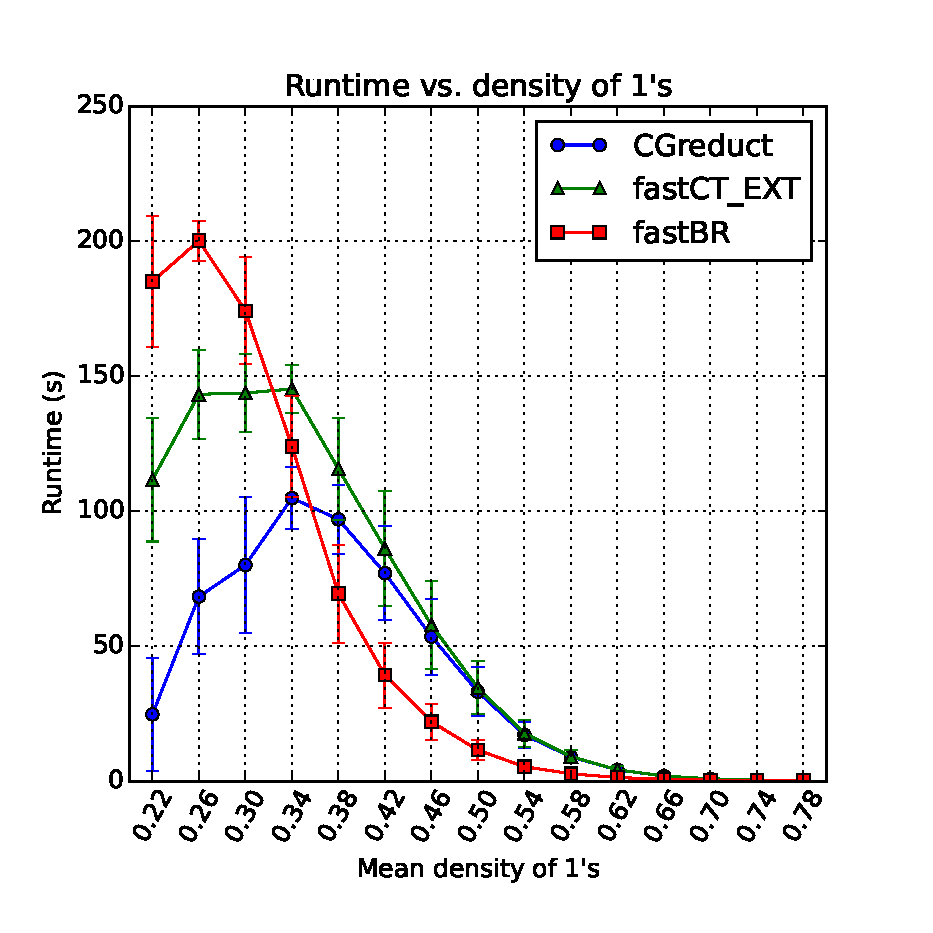
\includegraphics[height=8cm]{overal.eps}
	\end{center}
	\caption{Average algorithms' runtime vs. density of 1's for all synthetic \textit{SBDMs}.}
	\label{fig:scattDensity}
\end{figure}	

  For clarity purposes, the 500 matrices were split into 15 groups by discretizing the range of densities, each group having approximately 33 \textit{SBDMs}. Figure~\ref{fig:scattDensity} shows the average runtime of all  matrices in each group for the three algorithms, as a function of the density of 1's in the synthetic \textit{SBDMs}. In this figure, the vertical bars show the standard deviation of each bin. 

  From Figure~\ref{fig:scattDensity}, we can see that the fastest algorithm for matrices with density under 0.36 was GCreduct, fast--BR was the fastest for matrices with density between 0.36 and 0.66, and the three algorithms shown similar performance for matrices with density above 0.66. The fact that high density \textit{SBDMs} do not constitute a complex computational task for reduct computation \citep{Rojas12} is clearly visible in Figure~\ref{fig:scattDensity}. For this reason, a detailed analysis in this region lacks of relevance.

  In order to explain the line delimiting those \textit{SBDMs} for which GCreduct is faster than fast--BR (densities under 0.36), we must go deeply into the main difference between these algorithms. In GCreduct, we compute the exclusion mask and evaluate the attribute exclusion, only for those candidates detected as super-reducts; in order to verify whether they are reducts. In fast--BR, on the other hand, the attribute exclusion is evaluated for each candidate with a contributing attribute, mo matters whether it is a reduct. The evaluation of the attribute exclusion is the part with the highest computational complexity in both algorithms ($\Theta (nm)$). The attribute exclusion occurs when there is at least one column in the sub-matrix of the \textit{SBDM}, considering only the attributes in the current candidate, that can be removed without increasing the number of zero rows in this sub-matrix. The exclusion is more frequent in matrices with a higher density of 1's because the discernibility information is expressed by the 1's in the \textit{SBDM}, which have a greater overlapping for these kind of matrices. The higher cost of candidate evaluation in fast--BR pays off for \textit{SBDMs} with higher densities (the limit identified from our experiment is 0.36), because supersets of candidates with attribute exclusion are excluded from subsequent evaluations. Take for instance the extreme case of the identity matrix, where there is no exclusion at all, since every attribute is indispensable to form a reduct. For this kind of \textit{SBDMs}, GCreduct needs to evaluate as many candidates as fast--BR but our proposal makes a single verification for exclusion with the set of all attributes. On the other hand, fast--BR verifies the exclusion for each candidate, which leads to a higher computational cost.

  Friedman tests and post hoc Nemenyi-Damico-Wolfe-Dunn tests show that GCreduct was significantly faster (\textit{p--value} $< 10^{-16}$) than fast--CT\_EXT for low (under 0.36) and medium (between 0.36 and 0.66) density matrices. In relation to fast--BR, GCreduct showed a significant runtime reduction (\textit{p--value} $< 10^{-16}$) for low density matrices while it was significantly slower (\textit{p--value} $< 10^{-16}$) for medium density matrices. From this analysis, we conclude that GCreduct is the best algorithm for low density matrices; while fast--BR is the best for medium density matrices. For high (over 0.66) density matrices any algorithm can be used since, computing reducts on this kind of matrices does not constitute a complex computational task \citep{Rojas12}. Moreover, from these conclusions, a great advantage can be taken of selecting the appropriate algorithm for each dataset. 

\begin{table}[htb]
	\centering
	\caption{Fast--CText, GCreduct and Fast--BR runtime for standard datasets. Sorted by \textit{SBDM} density.}
	\label{tab:density}
	\begin{tabular}{|l|c|r|r|r|}
		\hline
		\multicolumn{1}{|c|}{Information}  && Fast--CText & \multicolumn{1}{c|}{Gcreduct} & \multicolumn{1}{c|}{Fast--BR}  \\
		\multicolumn{1}{|c|}{system}       & Density & runtime (s) & runtime (s)  & runtime (s)  \\
		\hline
		Chess (kr-vs-kp)          & 0.03    & 7.45          & \textbf{$<$0.01} & 0.02            \\
		Keyword-activity          & 0.04    & 1.22          & \textbf{0.42}    & 0.90            \\
		Connect-4                 & 0.05    & 12876.67      & \textbf{44.23}   & 160.61          \\
		QSAR-biodeg               & 0.12    & 0.75          & \textbf{0.19}    & 0.33            \\
		Landsat (train)           & 0.33    & 23797.99      & \textbf{9949.31} & 17732.49        \\
		Dermatology               & 0.34    & 16.02         & 12.25            & \textbf{4.62}   \\
		Credit-g                  & 0.35    & \textbf{0.05} & 0.06             & 0.12            \\
		Flags                     & 0.35    & 1.00          & \textbf{0.74}    & 1.06            \\
		Diabetes                  & 0.38    & 86.99         & \textbf{19.48}   & 23.37           \\
		Student-por               & 0.41    & 1874.57       & 1657.90          & \textbf{161.35} \\
		Sponge                    & 0.42    & 0.63          & 0.58             & \textbf{0.14}   \\
		Student-mat               & 0.43    & 1003.87       & 929.46           & \textbf{81.82}  \\
		Lung-cancer               & 0.47    & 188.20        & 133.43           & \textbf{7.34}   \\
		Waveform                  & 0.50    & 2.11          & 1.88             & \textbf{1.64}   \\
		Cylinder-bands            & 0.55    & 5.03          & 4.59             & \textbf{0.53}   \\
		\hline
	\end{tabular}
\end{table}

  In Table~\ref{tab:density} we included the density of 1's of the \textit{SBDMs} used to obtain the results shown in Table~\ref{tab:java}. We also sorted the datasets in Table~\ref{tab:density} in ascending order according to the density of 1's in their associated \textit{SBDM}. Although this is a small heterogeneous sample, the rule obtained from synthetic data can be verified in this table. For datasets with densities close to the boundary of 0.36 we cannot conclude a fastest algorithm as it can be seen in Table~\ref{tab:density}. However, for those datasets which have a \textit{SBDM} with density clearly under 0.36, GCreduct performed faster. In the same way, fast-BR performed faster for those datasets with density clearly above 0.36.

\section{Schedule}\label{sec_schedule}
  Table~\ref{tab_Schedule} shows the schedule of the main tasks that will be carried out throughout this research. The work to be done in the next evaluation period, is related in the schedule and listed bellow:

\section{Tasks for the next period}\label{sec_schedule}
  Table~\ref{tab_Schedule} shows the schedule of the main tasks that will be carried out throughout this research. As it can be seen, the executed tasks in the current period correspond to those related in Table~\ref{tab_Schedule}. In the same form, the work to be done in the next evaluation period is shown in the schedule and listed bellow:
  
  \begin{itemize}
  	\itemsep0em 
  	\item Literature review.
  	\item Critical study of algorithms for computing shortest reducts in information systems.
  	\item Implementation of algorithms for computing shortest reducts in information systems.
  	\item Experimental study on algorithms for computing shortest reducts in information systems.
  	\item Continue writing the PhD dissertation.
  \end{itemize}
  
  
 \begin{table}[h!]
		\caption{Research schedule (quarterly\protect\footnotemark).} \label{tab_Schedule}
		\centering
 	\begin{tabular}{|p{7cm}|c|c|c|c|c|c|c|c|c|c|c|c|}
 		\hline
		\multicolumn{1}{|c|}{\multirow{3}{*}{Task}} & \multicolumn{12}{c|}{Quarters}\\
 		\cline{2-13}
		 & 2014 & \multicolumn{3}{c|}{2015} & \multicolumn{3}{c|}{2016} & \multicolumn{3}{c|}{2017}
		 & \multicolumn{2}{c|}{2018} \\
 		\cline{2-13}
		 & 1 & 2 & 3 & 4 & 5 & 6 & 7 & 8 & 9 & 10 & 11 & 12 \\
		\hline
		Literature review &\cellcolor{blue}&\cellcolor{blue}&\cellcolor{blue}&
		\cellcolor{blue}&\cellcolor{blue}&\cellcolor{blue}&\cellcolor{blue}&
		\cellcolor{blue}&\cellcolor{blue}&\cellcolor[gray]{0.9}&\cellcolor[gray]{0.9}&
		\cellcolor[gray]{0.9}\\
		\hline
		Writing the research proposal &\cellcolor{blue}&\cellcolor{blue}&\cellcolor{blue}&&&&&&&&&\\
		\hline
		Critical study of algorithms for computing all reducts in information systems
		&\cellcolor{blue}&\cellcolor{blue}&\cellcolor{blue}&&&&&&&&&\\
		\hline
		Implementation of algorithms for computing all reducts in information systems
		&&\cellcolor{blue}&\cellcolor{blue}&&&&&&&&&\\
		\hline
		Development of a new algorithm for computing all reducts in information systems
		&&&&\cellcolor{blue}&&&&&&&&\\
		\hline
		Critical study of algorithms for computing shortest reducts in information systems
		&&&&\cellcolor{blue}&&\cellcolor{blue}&\cellcolor{blue}&\cellcolor{blue}&&&&\\
		\hline
		Implementation of algorithms for computing shortest reducts in information systems
		&&&&&&&\cellcolor{blue}&\cellcolor{blue}&&&&\\
		\hline
		Development of a new algorithm for computing shortest reducts in information systems
		&&&&&&&&\cellcolor{blue}&&&&\\
		\hline
		Critical study of hardware accelerations of algorithms for computing reducts in information systems
		&&&&&&&&&\cellcolor{blue}&\cellcolor[gray]{0.9}&&\\
		\hline
		Designing and implementing in hardware the proposed algorithms
		&&&&&&&&&\cellcolor{blue}&\cellcolor[gray]{0.9}&&\\
		\hline
		Experimental set-up &\cellcolor{blue}&\cellcolor{blue}&&\cellcolor{blue}&
		\cellcolor{blue}&&\cellcolor{blue}&\cellcolor{blue}&&&&\\
		\hline
		Experiments run &&&\cellcolor{blue}&\cellcolor{blue}&&\cellcolor{blue}&\cellcolor{blue}&&
		\cellcolor{blue}&&&\\
		\hline
		Writing papers &\cellcolor{blue}&&\cellcolor{blue}&&\cellcolor{blue}&\cellcolor{blue}&&&
		\cellcolor{blue}&&&\\
		\hline
		Writing the PhD dissertation &&&&\cellcolor{blue}&\cellcolor{blue}&\cellcolor{blue}&
		\cellcolor{blue}&\cellcolor{blue}&\cellcolor{blue}&&&\\
		\hline
		Submit final draft of the PhD dissertation to the advisors &&&&&&&&&&\cellcolor[gray]{0.9}&&\\
		\hline
		Submit final version of the PhD dissertation to the PhD committee &&&&&&&&&&&\cellcolor[gray]{0.9}&\\
		\hline
		
 	\end{tabular}             
 \end{table}
 
   Based on the results reported in this document, we can conclude that our goals can be reached into the expected time.
 \footnotetext{Quarters are: [January-April], [May-August] and [September-December]. Schedule starts in 
 			   September 2014, according to the admission of the student in the PhD program.}
	  	


	
%-------------------------------------------------------------------------------
% Bibliography
%-------------------------------------------------------------------------------

\bibliography{mybib}{}
\bibliographystyle{authordate1}
\end{document}
